\section{Estudo experimentao}
\label{sec:estudo}

	O estudo deste trabalho, nesta primeira fase, foi baseado nos seguintes ambientes de
rede social que utilizam a plataforma noosfero:
%
o portal Participa.Br\footnote{Participa.Br}, para as observações sobre a usabilidade do Noosfero;
%
a rede Comunidade.UnB\footnote{comunidade.unb.br} e o Portal UnB Gama\footnote{fga.unb.br}, para as observações sobre os testes automatizados no Noosfero;
%

Foi planejado um estudo de usabilidade, cujo o objetivo é analisar a interação dos usuários com o portal Participa.Br a fim de avaliar a qualidade em uso do portal. 
%
A partir dos objetivos de medição estabelecidos, foram definidas questões sobre o que é preciso saber de forma a apoiá-la a entender se o objetivo específico foi alcançado. Assim, para cada questão foram definidas as métricas relacionadas na Tabela~\ref{tabela-questoes}: 

\begin{table}[h]
\begin{tabular}{|l|l|l|}
\hline
\textbf{Questões}  & Métricas    & \begin{tabular}[c]{@{}l@{}}Diretrizes para \\ interpretação \end{tabular}  \\ \hline
\begin{tabular}[c]{@{}l@{}} Q1. Qual o perfil do usuário \\ que utiliza o  Participa.Br?  \end{tabular} &                Perfil               & \begin{tabular}[c]{@{}l@{}} Análise de Dados Estatísticos,\\ criação de personas, análise \\ dos dados qualitativos. \end{tabular}\\ \hline
\begin{tabular}[c]{@{	}l@{}} Q2. Qual o grau de satisfação\\ do usuário que utiliza o  \\ Participa.Br \end{tabular} &  \begin{tabular}[c]{@{}l@{}} Grau de satisfação \\ do usuário \end{tabular} & \begin{tabular}[c]{@{}l@{}} Escore da satisfação global\\ pelo usuário (OVERALL)   \end{tabular}                               \\ \hline
\begin{tabular}[c]{@{}l@{}} Q3. Quantidade de tempo gasto \\ para realizar as tarefas   \end{tabular}   &            Duração                   & Tempo gasto                       \\ \hline
\end{tabular}
\caption{Questões de Pesquisa}
\label{tabela-questoes}
\end{table}

Foram levantadas algumas hipóteses para este estudo experimental no Participa.Br:

\begin{enumerate}
\item A média do grau de satisfação dos usuários que já utilizaram o portal seria maior do que quem nunca utilizou?

\item O grau de satisfação dos usuários que já tinha contato com o portal é diferente dos que nunca tiveram acesso?
\end{enumerate}

Do ponto de vista de metodológico, elencamos algumas técnicas para identificamos o perfil dos usuários do Participa.Br:

\begin{enumerate}
\item \textbf{Dados Estatísticos} (\textit{Google analytcs}, Piwiki, entre outros): Através dos dados estatísticos é possível identificar algumas informações sobre o perfil dos usuários que acessam o portal. Nas pesquisas quantitativas não são necessários o contato direto com o usuário. Esses dados estatísticos podem ser coletados de base de dados, redes sociais ou sistemas de análises de sites.

\item \textbf{Questionário de identificação de perfil dos usuários:} Para identificar o perfil dos usuários do Portal da Participação social é necessário realizar uma pesquisa qualitativa para levantamento das principais características contextuais dos usuários típicos, de modo a compreender quem são, qual o conhecimento e experiência com a internet e como utilizam para realizar seu trabalho acadêmico ou profissional. A realização dessa pesquisa será feita com os usuários do Portal da Participação Social.
%
A análise do questionário servirá para entender o perfil dos usuários do Portal da participação social, através da investigação de seus interesses. Foi levantado também algumas questões referentes ao uso das funcionalidades do Participa.Br.

\item \textbf{Identificação de Personas:} Para a definição de usuários podemos utilizar a técnica de “Persona” que são personagens fictícios criados com base em dados reais. Os Personas atuam como representantes dos usuários reais e representam as necessidades de um grupo maior. 
%
\end{enumerate}
Elencamos algumas técnicas para avaliar a usabilidade do portal Participa.Br:

\begin{table}[h]
\begin{tabular}{|l| p{10cm} |}
\hline
Técnica & Descrição \\ \hline
Observar Usuários & Um observador irá registrar o tempo 
gasto por cada participante para concluir o estudo de caso, 
avaliar a ferramenta e se necessitou de alguma ajuda    \\ \hline
Perguntar aos usuários & Os questionários ASQ e PSSUQ 
de satisfação dos usuários será utilizado 
para coletar as opiniões dos participantes.\\ \hline
\end{tabular}
\caption{Técnicas de avaliação para os testes com usuários}
\end{table}

Os instrumentos de coletas de informações utilizados são dois questionários que são amplamente utilizados para medir a satisfação do usuário com produtos interativos e fornecem medidas padronizadas.
%
São eles o \textit{After-Scenario Questionnaire} (ASQ) \footnote{ASQ: Proposto por Lewis} e o \textit{Post-Study System Usabiliy Questionnaire} (PSSUQ). 
%
O ASQ é destinado ao uso em testes de usabilidade baseados em cenários. Possui três itens que abordam os seguintes componentes de usabilidade: (1) facilidade de conclusão da tarefa, (2) tempo necessário para completar uma tarefa e,(3) a adequação das instruções ou materiais de apoio fornecidos.
%
O PSSUQ é aplicado após a conclusão de todos os cenários com o propósito de fornecer uma avaliação geral geral da usabilidade do sistema. pois permite uma avaliação de usabilidade mais ampla, podendo avaliar 4 fatores e usabilidade (satisfação geral, utilidade do sistema, qualidade da interface e qualidade da informação). 

%+++++++++++++++++++++++++++++++++++++++++++++++++++++++++++++++++++++++++++++++++++++++++++%

O estudo sobre testes teve seu enfoque na rede colaborativa baseada 
no noosfero desenvolvida para a Universidade de Brasília (UnB)\footnote{\url{unb.br}}. Ao decorrer deste trabalho de graduação, foram desenvolvidos, juntamente com seus respectivos testes, alguns \textit{plugins} que serão descritos nesta seção.

Como rede colaborativa dos membros da Universidade de Brasília, o Comunidade UnB 
necessita possuir restrição de acesso aos usuários, para que somente membros ativos 
da universidade tenham acesso ao conteúdo da rede colaborativa. 
%
Para que esta necessidade fosse satisfeita foi desenvolvido um \textit{plugin} no noosfero, que efetuasse as restrições necessárias, utilizando o protocolo de autenticação da UnB, o LDAP (\textit{Lightweight Directory Access Protocol}).

Com o auxílio de uma ferramenta de análise de código para \textit{Ruby} chamada Rcov, foi obtida a taxa de cobertura de código do \textit{plugin} desenvolvido, além de alguns dados sobre a execução dos testes funcionais e unitários que seguem abaixo:

\begin{itemize}
\item Quantidade de testes executados: \textbf{96 testes;}
\item Quantidade de assertivas executadas: \textbf{111 assertivas;}
\item Quantiadde de falhas obtidas: \textbf{0 falhas;}
\item Tempo de execução dos testes: \textbf{7.8 segundos;}
\end{itemize}

Na imagem \ref{consideracoes_cobertura1} existem dois gráficos de cobertura de código, o primeiro definido como \textit{'total coverage'} representa a contagem realizada com as linhas em branco e os comentários do código, já o \textit{'code coverage'} representa a contagem realizada sem as linhas em branco e os comentários do código.


\begin{figure}[!h]
    \centering
    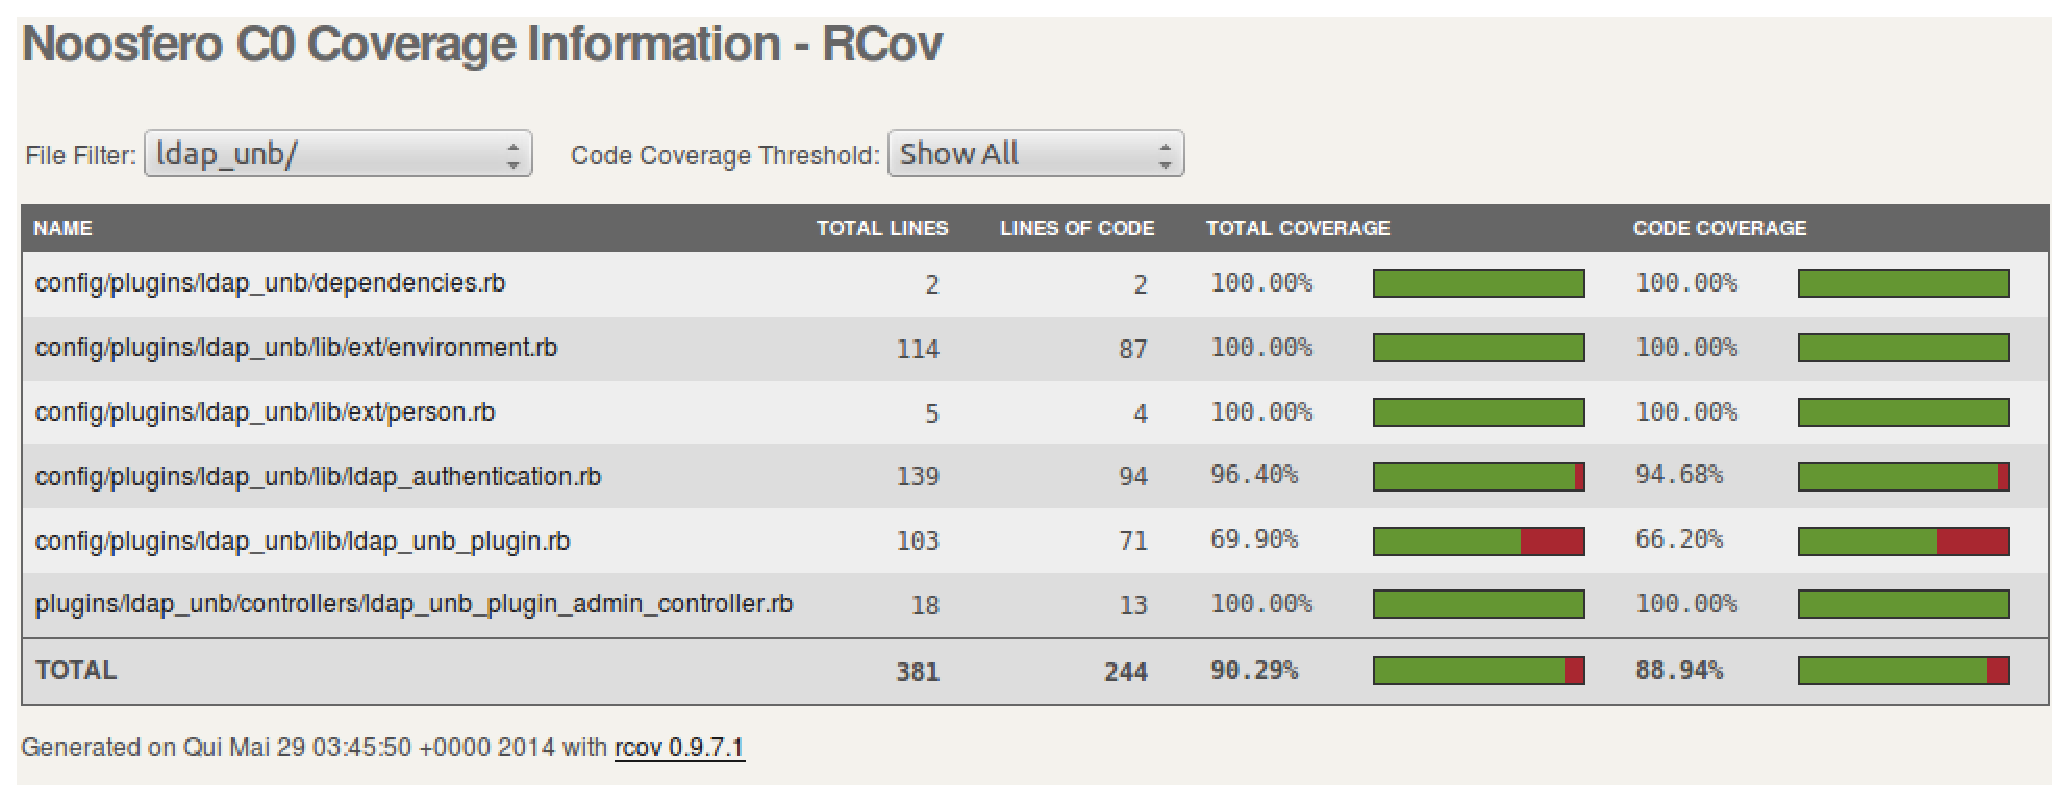
\includegraphics[keepaspectratio=false,scale=0.45]
      {images/cobertura_teste.eps}
    \caption{Cobertura de código do plugin LdapUnb}
    \label{consideracoes_cobertura1}
\end{figure}

Este \textit{plugin} também foi desenvolvido para a plataforma Noosfero, porém em uma aplicação diferente, o Portal UnB Gama. A ideia deste \textit{plugin} surgiu da necessidade de existir um ambiente virtual em que os trabalhos de conclusão de curso pudessem ser submetidos aos professores e compartilhados com a comunidade acadêmica, buscando assim manter uma forma de versionamento dos trabalhos desenvolvidos e dispensando a necessidade de trabalhos de conclusão de curso impressos.
%
Este \textit{plugin} é responsável por criar uma atribuição de trabalhos, chamada de \textit{work assignment}. Essa atribuição possui algumas funcionalidades específicas como possibilitar que os usuários envolvidos sejam notificados via \textit{email} sobre a submissão de um certo trabalho. Para tal foi necessário instanciar um servidor de \textit{email} para executar estas notificações, assim como criar uma página no Portal FGA\footnote{url{fga.unb.br}} para que o usuário pudesse submeter seu trabalho.
%


A ferramenta Rcov também foi utilizada para dimensionar a taxa de cobertura de código do \textit{plugin} para envio de TCC, segue os dados sobre a execução dos testes funcionais e unitários:

\begin{itemize}
\item Quantidade de testes executados: \textbf{28 testes};
\item Quantidade de assertivas executadas: \textbf{84 assertivas};
\item Quantiadde de falhas obtidas: \textbf{0 falhas};
\item Tempo de execução dos testes: \textbf{10,5 segundos};
\end{itemize}

Na imagem \ref{consideracoes_cobertura2} está representado a cobertura de código, extraída da ferramenta Rcov:

\begin{figure}[!h]
    \centering
    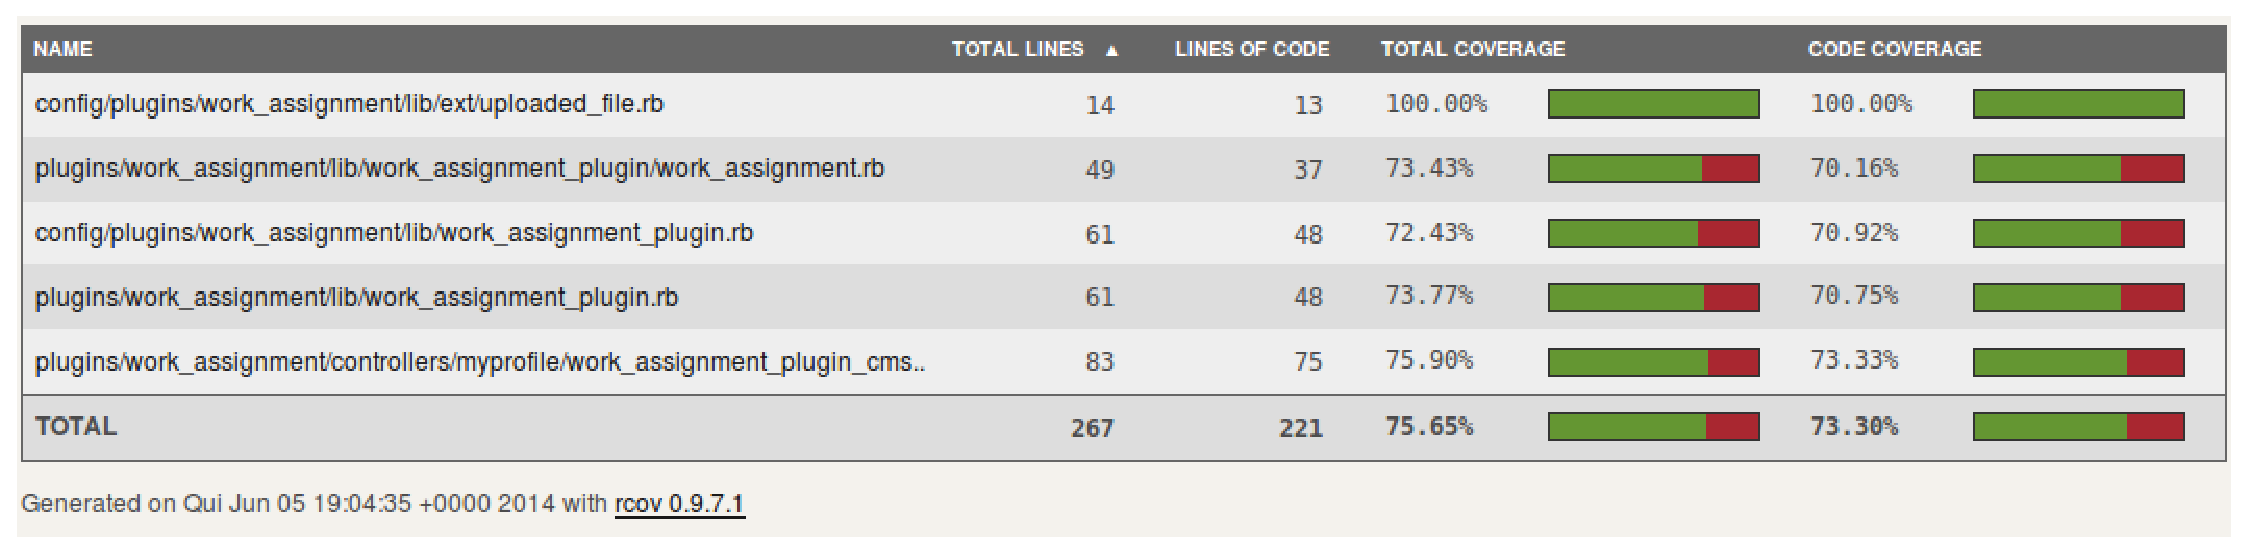
\includegraphics[keepaspectratio=false,scale=0.45]
      {images/cobertura_tcc.eps}
    \caption{Cobertura de código do plugin para submissão de trabalho}
    \label{consideracoes_cobertura2}
\end{figure}

Após a execução dos testes desenvolvidos, obtivemos os seguintes dados:

\begin{itemize}
\item Quantidade de cenários executados: \textbf{6 cenários};
\item Quantidade de passos executadas: \textbf{130 passos};
\item Quantiadde de falhas obtidas: \textbf{0 falhas};
\item Tempo de execução dos testes: \textbf{7 minutos e 18 segundos};
\end{itemize}


O desenvolvimento de testes automatizados é uma prática constante no desenvolvimento da plataforma noosfero e importante na validação de novos recursos desenvolvidos. Assim conseguimos verificar que a utilização de práticas de TDD e BDD como base para o desenvolvimento trouxe resultados satisfatórios, como será mostrado no capítulo a seguir.

Com a proposta de algumas técnicas de avaliação da usabilidade para o Portal da Participação Social, verificamos que muitas delas precisam ser adaptadas para uma melhor adoção nos ambientes de software livre e em métodos ágeis. O teste de usabilidade proposto foi planejado pensando nas práticas clássicas de avaliação da usabilidade que é considerada por vários autores como uma das melhores maneiras de avaliar uma interface.